\documentclass{beamer}
%\usetheme{Madrid}
\usecolortheme{rose}
%\usefonttheme{serif}
\usepackage[utf8]{inputenc}
\usepackage[spanish]{babel}
\usepackage{graphicx}
\usepackage{amsmath} % Paquete para ecuaciones

\title{Sistema de Navegación Adaptativa para un Vehículo Autónomo}
\author{
    Over Alexander Mejia Rosado \\
    Ronald Mateo Ceballos Lozano \\
    Rhonald José Torres Díaz
}
\institute{\textit{Inteligencia Artificial} \\
Universidad Nacional de Colombia - De La Paz}
\date{}

\begin{document}

\begin{frame}
    \titlepage
\end{frame}

\begin{frame}{Introducción}
    \begin{itemize}
        \item Desarrollo de un vehículo autónomo capaz de desplazarse en un mapa 2D.
        \item Implementación del algoritmo NEAT (NeuroEvolution of Augmenting Topologies).
        \item Uso de sensores virtuales para la percepción del entorno.
        \item Aplicación de métricas de distancia (Euclidiana, Manhattan, Chebyshev) como sistema de recompensas.
        \item Creación de un sistema de refuerzo para evitar el estancamiento del vehículo.
    \end{itemize}
\end{frame}

\begin{frame}{Objetivo del Proyecto}
    \begin{itemize}
        \item Determinar que metricas de distancia son mas efectivas para el cálculo del fitness.
        \item Utilizar NEAT (NeuroEvolution of Augmenting Topologies) para desarrollar el sistema de navegación.
        \item Mejorar la capacidad del vehículo de adaptarse al entorno.
    \end{itemize}
\end{frame}

\section{Metodología}

\begin{frame}{Metodología}
    \begin{itemize}
        \item Creación del entorno 2D con la herramienta Pygame Python.
        \item Uso de métricas de distancia (Euclidiana, Manhattan, Chebyshev) como sistema de recompensas.
        \item Creación de un sistema de un metodo para evitar que el vehículo se estanque.
    \end{itemize}
\end{frame}

\begin{frame}{Entorno 2D}
    \begin{columns}
        \begin{column}{0.5\textwidth}
            \begin{figure}
                \centering
                % Primera imagen (dentro del directorio actual)
                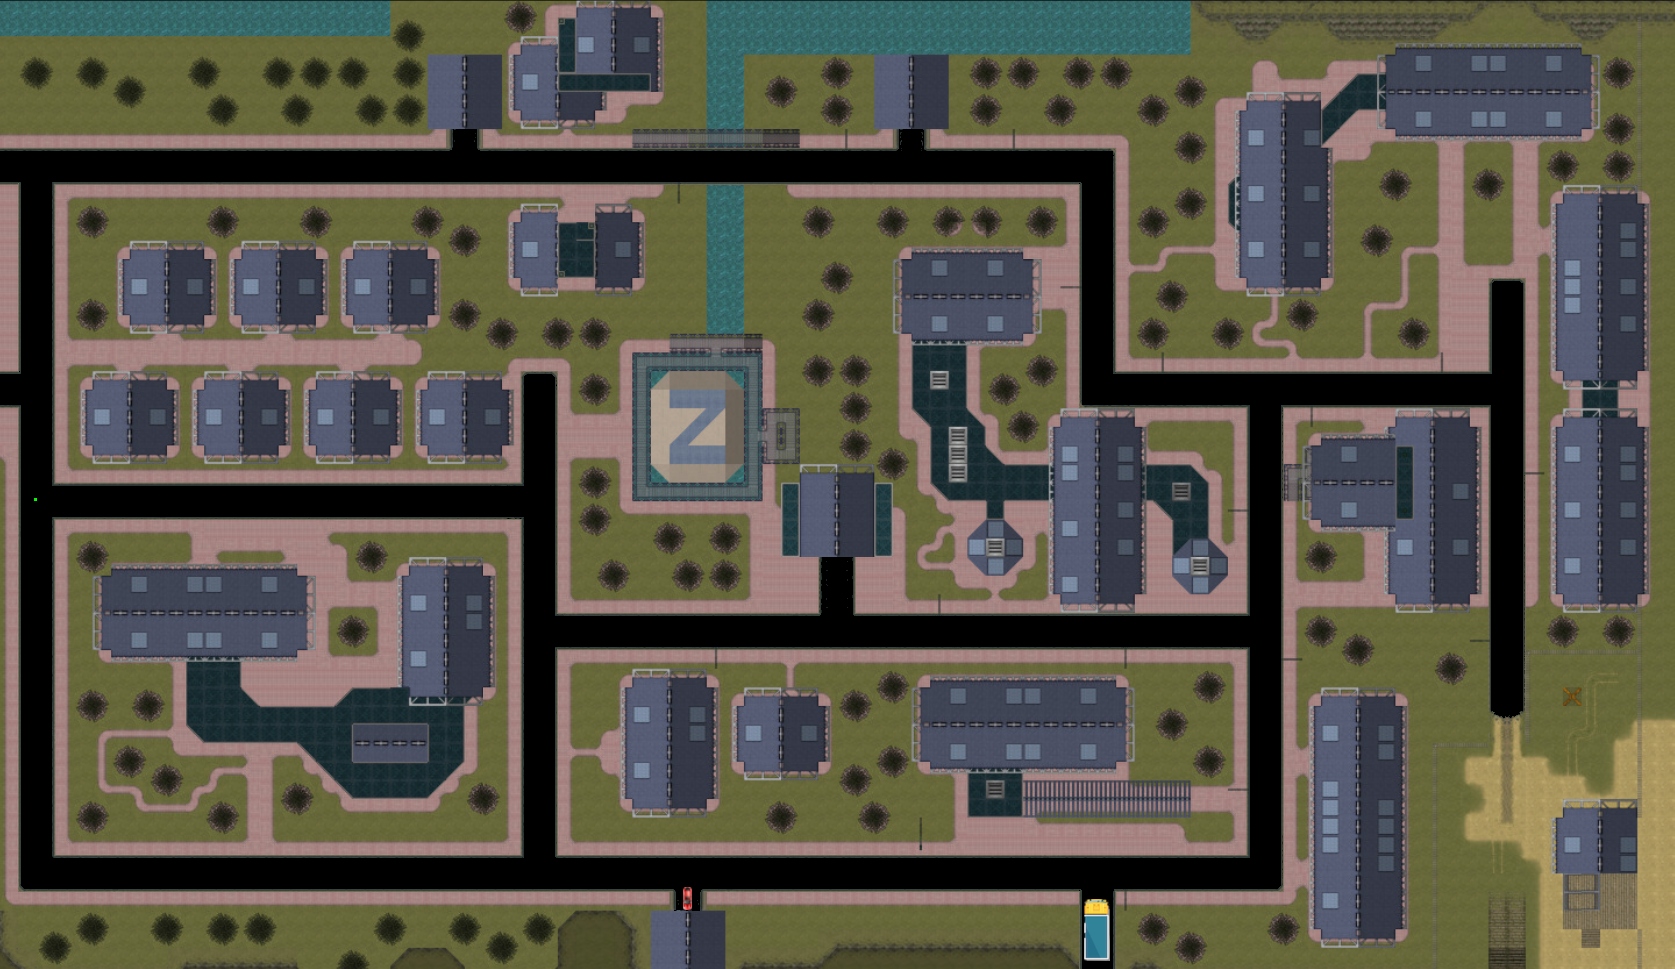
\includegraphics[width=\linewidth]{images/gta2.png}
            \end{figure}
            \vspace{0.5cm} % Espacio entre las imágenes
            \begin{figure}
                \centering
                % Segunda imagen (una carpeta atrás)
                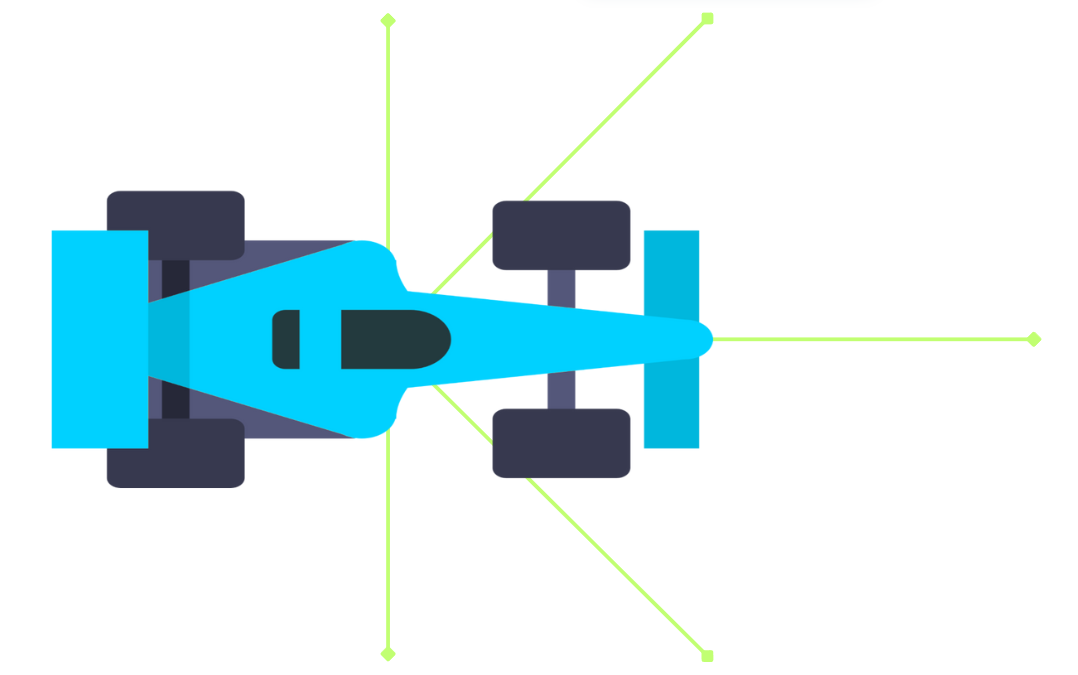
\includegraphics[width=\linewidth]{images/sensores.png}
            \end{figure}
        \end{column}
        \begin{column}{0.5\textwidth}
            \begin{itemize}
                \item Mapa 2D implementado en las simulaciones realizadas.
                \item Aplicacion de radares al agente.
                \item .
            \end{itemize}
        \end{column}
    \end{columns}
\end{frame}

\begin{frame}{Metodología}

\textbf{Cálculo del Fitness}

Utilizamos diferentes métricas de distancia para calcular el fitness del vehículo autónomo. La función de fitness se define como:

\[
\text{Fitness} = \max\left(0,\  10000 - d \right)
\]

Donde \( d \) es la distancia calculada según la métrica utilizada.

\textbf{Métricas de Distancia}
\begin{itemize}
  \item \textbf{Distancia Euclidiana}:
  \[
  d_{\text{E}} = \sqrt{(x_{\text{meta}} - x_{\text{veh}})^2 + (y_{\text{meta}} - y_{\text{veh}})^2}
  \]
  
\end{itemize}

\end{frame}

\begin{frame}{Metodología}
  \begin{itemize}
    \item \textbf{Distancia de Manhattan}:
  \[
  d_{\text{M}} = |x_{\text{meta}} - x_{\text{veh}}| + |y_{\text{meta}} - y_{\text{veh}}|
  \]
  
    \item \textbf{Distancia de Chebyshev}:
    \[
    d_{\text{C}} = \max\left( |x_{\text{meta}} - x_{\text{veh}}|,\  |y_{\text{meta}} - y_{\text{veh}}| \right)
    \]
  \end{itemize}
 

\textbf{Sensores Virtuales}

Los sensores proporcionan información sobre el entorno inmediato del vehículo, incluyendo obstáculos y límites de la vía.

\end{frame}

\begin{frame}{Metodología}

  \textbf{Algoritmo NEAT}

Se utiliza NEAT para evolucionar la arquitectura de la red neuronal que controla el vehículo. NEAT permite:

\begin{itemize}
    \item Incrementar complejidad de la red gradualmente.
    \item Preservar estructuras efectivas a través de la especiación.
\end{itemize}


  \textbf{Refuerzo Forzado}

Para evitar que el vehículo se estanque, se implementa una mecánica donde, si la velocidad es inferior a un umbral, se aplica un impulso para mantener el movimiento.

\end{frame}

\begin{frame}{NEAT (NeuroEvolution of Augmenting Topologies)}
    \begin{itemize}
        \item Algoritmo evolutivo para el desarrollo de redes neuronales.
        \item Evoluciona tanto los pesos como la topología de las redes.
        \item Permite la adaptación y optimización continua del vehículo autónomo.
    \end{itemize}
\end{frame}

\begin{frame}{Resultados}
    \begin{itemize}
        \item El vehículo autónomo es capaz de desplazarse en el mapa de forma autónoma.
        \item Incremento del fitness en cada generación según la métrica de distancia utilizada.
        \item Mejora en la adaptabilidad y eficiencia del sistema de navegación.
    \end{itemize}
\end{frame}

\begin{frame}{Conclusiones}
    \begin{itemize}
        \item El uso de NEAT es efectivo para desarrollar sistemas de navegación adaptativos.
        \item Las métricas de distancia y el refuerzo forzado contribuyen al aprendizaje del vehículo.
        \item Potencial para reducir accidentes y mejorar la eficiencia en sistemas de transporte autónomo.
    \end{itemize}
\end{frame}

\begin{frame}{Preguntas}
    \centering
    {\Huge ¿Preguntas?}
\end{frame}

\end{document}